\documentclass[12pt,a4paper]{article}
\usepackage[utf8]{inputenc}
\usepackage{amsmath, amssymb, amsthm} 
\usepackage{graphicx}
\usepackage{hyperref}
\usepackage{geometry}
\usepackage{listings} % Pentru un afișaj mai bun al codului
\usepackage{xcolor} % Pentru culori în listings

\geometry{margin=2.5cm}

% Configurare pentru listings (opțional, dar arată mai bine)
\lstset{
	language=Python,
	basicstyle=\ttfamily\footnotesize,
	keywordstyle=\color{blue},
	commentstyle=\color{green!40!black},
	stringstyle=\color{purple},
	showstringspaces=false,
	breaklines=true,
	frame=tb, % Doar linii sus și jos pentru un aspect mai curat
	framesep=5pt,
	framexleftmargin=1pt,
	numbers=left,
	numberstyle=\tiny\color{gray},
	tabsize=4,
	captionpos=b % Poziția caption-ului sub listing
}


\title{Sistem de recomandare folosind factorizare de matrice și similaritate pe taguri}
\author{Gatej Stefan-Alexandru, Potop Horia-Ioan}
\date{\today} % Sau \date{Mai 2024} etc.

\begin{document}
	
	\maketitle
	\tableofcontents
	\newpage
	
	\section{Descrierea aplicației}
	
	Scopul acestei componente a sistemului de recomandare este de a genera recomandări de melodii similare pe baza caracteristicilor extrase din tagurile asociate fiecărei piese muzicale. Problema centrală abordată este factorizarea unei matrice binare (melodie $\times$ tag) într-un spațiu latent de dimensiune redusă, sub constrângeri de non-negativitate. Această factorizare permite descoperirea unor structuri și similarități ascunse între melodii, care pot fi apoi utilizate pentru a genera recomandări personalizate.
	
	\section{Formularea matematică a problemei de factorizare}
	
	Problema de bază pentru metodele de factorizare de matrice (NMF, ALS-NNLS) este următoarea:
	Fie $V \in \mathbb{R}^{m \times n}$ matricea de intrare (în cazul nostru, matricea binară melodie $\times$ tag), unde $m$ este numărul de melodii și $n$ este numărul de taguri unice. Dorim să găsim două matrice, $W \in \mathbb{R}^{m \times r}$ (matricea factorilor latenti pentru melodii) și $H \in \mathbb{R}^{r \times n}$ (matricea factorilor latenti pentru taguri), unde $r \ll \min(m,n)$ este dimensiunea spațiului latent (numărul de factori).
	
	Problema de optimizare este de a minimiza eroarea de reconstrucție, adesea măsurată prin norma Frobenius pătrată:
	
	\begin{equation}
		\min_{W, H} \| V - W H \|_F^2
		\label{eq:nmf_objective_main}
	\end{equation}
	
	\textbf{Constrângeri de Non-Negativitate:}
	Pentru a asigura interpretabilitatea factorilor și pentru a se alinia cu natura aditivă a multor date (cum ar fi prezența tagurilor sau numărul de ascultări), se impun constrângeri de non-negativitate:
	\begin{itemize}
		\item $W_{ij} \geq 0$ pentru toți $i,j$
		\item $H_{ij} \geq 0$ pentru toți $i,j$
	\end{itemize}
	Aceste constrângeri transformă problema într-una de optimizare cu constrângeri.
	
	\subsection{Alegerea numărului de factori latenti ($r$)}
	\label{subsec:alegerea-r}
	
	Numărul de factori latenti, $r$, este un hiperparametru crucial în algoritmii de factorizare de matrice, deoarece determină dimensionalitatea spațiului latent în care datele sunt proiectate. O valoare prea mică pentru $r$ poate duce la un model sub-antrenat (underfitting) care nu capturează suficientă informație din datele originale, rezultând într-o eroare de reconstrucție mare și recomandări de calitate inferioară. Pe de altă parte, o valoare prea mare pentru $r$ poate duce la supra-antrenare (overfitting), unde modelul începe să memoreze zgomotul specific setului de date de antrenament și nu generalizează bine pe date noi. De asemenea, un $r$ mare crește complexitatea computațională a antrenării și a utilizării modelului.
	
	În cadrul acestui proiect, pentru a permite o comparație directă și consistentă între diferitele metode de factorizare implementate (NMF Multiplicativ, NMF \texttt{sklearn}, ALS-NNLS Manual), am optat pentru o valoare fixă $r = 10$. Această valoare a fost aleasă ca un punct de pornire rezonabil pentru a demonstra funcționalitatea algoritmilor pe setul de date disponibil (\texttt{music\_info.csv}), permițând în același timp timpi de execuție gestionabili, în special pentru implementările manuale care sunt mai intensive computațional.
	
	Într-o aplicație practică sau într-un studiu mai aprofundat, selectarea optimă a lui $r$ ar necesita o abordare mai sistematică, implicând experimentarea cu o gamă de valori pentru $r$ și evaluarea performanței modelului folosind metrici adecvate. Metodele comune includ:
	\begin{itemize}
		\item \textbf{Monitorizarea erorii de reconstrucție:} Se analizează cum evoluează eroarea de reconstrucție (de ex., norma Frobenius a diferenței $V - WH$) pe măsură ce $r$ crește. Se caută adesea un punct de inflexiune ("cot" sau "elbow point") în graficul erorii vs. $r$, dincolo de care adăugarea de noi factori nu mai aduce o reducere semnificativă a erorii.
		\item \textbf{Metrici de evaluare specifice sarcinii:} Dacă scopul final este recomandarea și sunt disponibile date de feedback ale utilizatorilor (ex: ratinguri, istoric de ascultare), se pot utiliza metrici de ranking precum Precision@k, Recall@k, NDCG (Normalized Discounted Cumulative Gain) sau MAP (Mean Average Precision) pe un set de date de validare sau test. Valoarea lui $r$ care maximizează aceste metrici ar fi preferată.
		\item \textbf{Stabilitatea factorizării:} Se poate evalua cât de stabile sunt factorizările obținute pentru aceeași valoare $r$ la rulări multiple cu inițializări aleatorii diferite. O stabilitate mai mare este de dorit.
		\item \textbf{Interpretabilitatea factorilor:} În unele aplicații, se preferă un $r$ care produce factori latenti (coloanele lui $W$ sau liniile lui $H$) care au o interpretare semantică clară și relevantă pentru experții în domeniu.
	\end{itemize}
	Pentru scopurile acestei lucrări, ne-am concentrat pe compararea fundamentală a algoritmilor de optimizare cu constrângeri pentru un $r$ fix, recunoscând că optimizarea detaliată a acestui hiperparametru este un pas important, dar distinct, într-un scenariu de dezvoltare a unui sistem de recomandare de producție.
	
	\subsection{Rolul matricelor $W$ și $H$ în sistemul de recomandare}
	În urma procesului de factorizare, obținem două matrice, $W$ și $H$, care au interpretări și utilizări distincte în contextul recomandărilor:
	
	\begin{itemize}
		\item \textbf{Matricea $W \in \mathbb{R}^{m \times r}$ (Melodii $\times$ Factori Latenți):} Fiecare linie $W_i$ din această matrice reprezintă \textbf{profilul latent} al melodiei $i$. Acest vector $r$-dimensional încorporează caracteristicile "ascunse" ale melodiei, așa cum au fost ele învățate de algoritm. Pentru recomandările de tip melodie-melodie, așa cum sunt implementate în acest proiect, similaritatea dintre aceste profiluri latente (de exemplu, similaritatea cosinus între $W_i$ și $W_j$) este utilizată pentru a identifica melodii similare. Astfel, $W$ este matricea principală utilizată direct în funcția de generare a recomandărilor.
		
		\item \textbf{Matricea $H \in \mathbb{R}^{r \times n}$ (Factori Latenți $\times$ Taguri):} Această matrice leagă factorii latenti de tagurile originale. Fiecare coloană $H_j$ poate fi interpretată ca profilul latent al tagului $j$, iar fiecare linie $H_k$ arată importanța sau "încărcătura" factorului latent $k$ pentru fiecare tag original. Matricea $H$ este crucială pentru:
		\begin{itemize}
			\item \textbf{Interpretarea factorilor latenți:} Analizând liniile lui $H$, putem încerca să dăm un sens semantic fiecărui factor latent (ex: un factor ar putea fi puternic asociat cu taguri de "rock clasic", altul cu "muzică electronică ambientală").
			\item \textbf{Recomandarea de taguri pentru melodii:} Produsul $W_i H$ poate fi folosit pentru a prezice relevanța tagurilor pentru melodia $i$.
			\item \textbf{Găsirea de taguri similare:} Similaritatea dintre coloanele lui $H$ poate identifica taguri care sunt conceptual apropiate în spațiul latent.
			\item \textbf{Calitatea factorizării:} Ambele matrice, $W$ și $H$, sunt esențiale pentru reconstrucția $V \approx WH$ și, implicit, pentru calitatea generală a modelului.
		\end{itemize}
	\end{itemize}
	Deși funcția noastră principală de recomandare utilizează direct matricea $W$, matricea $H$ este o componentă indispensabilă a procesului de învățare și oferă posibilități valoroase de analiză și extindere a sistemului.
	
	\subsection*{Concepte cheie: Profil latent și Cluster latent}
	
	\paragraph{Profil latent}
	Un profil latent este o reprezentare numerică (un vector) a unei entități (de exemplu, o melodie) în spațiul de factori ascunși de dimensiune $r$, descoperit de algoritmul de factorizare. Liniile matricei $W$ (adică $W_i$) reprezintă aceste profiluri latente pentru melodii. Acești factori nu sunt direct observați în datele inițiale, ci sunt învățați pentru a surprinde structuri subiacente. De exemplu, un factor ar putea corespunde unui "grad de energie" al melodiei, altul unui "stil vocal specific", etc., chiar dacă aceste concepte nu sunt taguri explicite.
	
	\paragraph{Cluster latent}
	Un cluster latent se referă la un grup de entități (melodii) care au profiluri latente similare, adică sunt apropiate în spațiul latent $r$-dimensional. Deși nu aplicăm explicit un algoritm de clustering separat după NMF/ALS în această componentă pentru a defini clustere discrete, ideea este că melodiile cu vectori $W_i$ similari sunt considerate conceptual parte dintr-un "cluster" sau o regiune densă în spațiul latent. Recomandările se bazează pe această proximitate.
	
	\vspace{0.5em}
	\textit{Pe scurt: Profilul latent este vectorul de factori ascunși care descrie o melodie, iar similaritatea dintre aceste profiluri stă la baza recomandărilor bazate pe factorizare.}
	\vspace{1em} 
	
	\section{Soluții implementate pentru factorizarea cu constrângeri}
	
	Am implementat și comparat trei algoritmi pentru rezolvarea problemei de factorizare de matrice cu constrângeri de non-negativitate, așa cum este definită în ecuația (\ref{eq:nmf_objective_main}):
	
	\subsection{Algoritmul multiplicativ pentru NMF (NMF-MULT)}
	Acesta este un algoritm clasic pentru NMF, propus de Lee și Seung. El actualizează iterativ matricele $W$ și $H$ folosind următoarele reguli multiplicative, care garantează non-creșterea funcției obiectiv și menținerea non-negativității:
	\begin{align}
		H_{kj} &\leftarrow H_{kj} \frac{(W^T V)_{kj}}{(W^T W H + \epsilon)_{kj}} \\
		W_{ik} &\leftarrow W_{ik} \frac{(V H^T)_{ik}}{(W H H^T + \epsilon)_{ik}}
	\end{align}
	unde $\epsilon$ este o constantă mică (ex: $10^{-10}$) pentru a asigura stabilitatea numerică și a evita diviziunea cu zero.
	\begin{itemize}
		\item \textbf{Avantaje:} Simplu de implementat, relativ rapid pentru multe seturi de date, nu necesită alegerea unei rate de învățare.
		\item \textbf{Dezavantaje:} Poate converge lent, în special aproape de soluție, și este garantat să conveargă doar la un punct staționar, care poate fi un minim local.
	\end{itemize}
	
	\subsection{NMF din scikit-learn (\texttt{sklearn.decomposition.NMF})}
	Am utilizat implementarea NMF din biblioteca \texttt{scikit-learn}, care oferă mai mulți solveri. Am ales solver-ul \texttt{'cd'} (Coordinate Descent), care este eficient și adesea converge mai rapid decât regulile multiplicative simple pentru anumite tipuri de date, minimizând aceeași funcție obiectiv sub constrângeri de non-negativitate.
	\begin{itemize}
		\item \textbf{Avantaje:} Implementare optimizată (adesea în C/Cython), robustă, cu opțiuni pentru diferite inițializări și regularizări (deși nu le-am explorat în detaliu în această comparație de bază).
		\item \textbf{Solver ('cd'):} Algoritmul Coordinate Descent actualizează iterativ fiecare element (sau coloană/linie) dintr-o matrice (ținând cealaltă matrice fixă) prin rezolvarea unei subprobleme de optimizare univariată (sau de dimensiune mică).
	\end{itemize}
	
	\subsection{Alternating Least Squares cu Non-Negative Least Squares Manual (ALS-NNLS)}
	ALS este o altă abordare populară pentru factorizarea de matrice. Algoritmul optimizează alternativ pentru $W$ (ținând $H$ fix) și apoi pentru $H$ (ținând $W$ fix), minimizând funcția obiectiv (\ref{eq:nmf_objective_main}) la fiecare pas. Fiecare subproblemă devine o problemă de least squares. Pentru a impune constrângerile de non-negativitate, fiecare subproblemă de least squares este rezolvată ca o problemă de Non-Negative Least Squares (NNLS).
	\begin{itemize}
		\item \textbf{Subproblema pentru $W$ (pentru fiecare linie $W_i$):}
		$$ \min_{W_i \ge 0} \| V_i - W_i H \|_F^2 $$
		\item \textbf{Subproblema pentru $H$ (pentru fiecare coloană $H_{\cdot j}$):}
		$$ \min_{H_{\cdot j} \ge 0} \| V_{\cdot j} - W H_{\cdot j} \|_F^2 $$ 
	\end{itemize}
	Am implementat manual atât logica ALS, cât și un solver NNLS bazat pe metoda proiectării gradientului.
	\paragraph{NNLS Manual (Proiectarea Gradientului):}
	Pentru a rezolva $\min_{x \ge 0} \frac{1}{2}\|Ax - b\|_2^2$:
	\begin{enumerate}
		\item Se inițializează $x \ge 0$.
		\item Se calculează gradientul funcției obiectiv: $\nabla_x L(x) = A^T (Ax - b)$.
		\item Se face un pas în direcția opusă gradientului: $x \leftarrow x - \eta \nabla_x L(x)$, unde $\eta$ este rata de învățare.
		\item Se proiectează $x$ înapoi pe domeniul fezabil (elemente non-negative): $x_k \leftarrow \max(0, x_k)$ pentru fiecare componentă $k$.
		\item Se repetă pașii 2-4 până la convergență (ex: schimbarea în $x$ este sub o toleranță sau se atinge un număr maxim de iterații).
	\end{enumerate}
	\begin{itemize}
		\item \textbf{Avantaje:} Demonstrează înțelegerea detaliată a optimizării cu constrângeri și a descompunerii problemei. Permite control fin asupra procesului de optimizare a subproblemelor.
		\item \textbf{Dezavantaje:} Implementarea manuală (mai ales NNLS) poate fi lentă și sensibilă la parametrii precum rata de învățare și numărul de iterații interne NNLS.
	\end{itemize}

	
	\section{Rezultate numerice și concluzii}
	
	\subsection{Analiza convergenței și a erorilor de reconstrucție}
	\label{subsec:convergenta-erori}
	
	Performanța algoritmilor de factorizare este evaluată prin eroarea de reconstrucție și prin modul în care aceasta evoluează pe parcursul iterațiilor. Toate experimentele au fost rulate pentru $r=10$ factori latenti.
	
	\paragraph{NMF Multiplicativ (Manual):}
	Algoritmul NMF multiplicativ a prezentat o scădere monotonă a erorii de reconstrucție, așa cum era de așteptat:
	\begin{verbatim}
		Multiplicative NMF Iteration 0: error = 403.9834
		Multiplicative NMF Iteration 10: error = 350.3428
		...
		Multiplicative NMF Iteration 90: error = 337.0462
	\end{verbatim}
	Eroarea finală raportată a fost de \textbf{337.03}.
	
	\paragraph{NMF (\texttt{sklearn}, solver 'cd'):}
	Implementarea din \texttt{sklearn} a raportat direct o eroare finală de reconstrucție de \textbf{336.42}, fiind cea mai mică dintre metodele testate.
	
	\paragraph{ALS cu NNLS Manual (ALS-NNLS):}
	Pentru implementarea ALS cu subprobleme NNLS rezolvate manual, evoluția erorii a fost următoarea:
	\begin{verbatim}
		ALS-NNLS Iteration 0: Frobenius error = 393.1052
		ALS-NNLS Iteration 5: Frobenius error = 342.6145
		ALS-NNLS Iteration 10: Frobenius error = 339.7412
		ALS-NNLS Iteration 15: Frobenius error = 339.2437
		ALS-NNLS Iteration 20: Frobenius error = 339.1804
		ALS-NNLS Iteration 25: Frobenius error = 339.1712
		ALS-NNLS converged at iteration 28.
	\end{verbatim}
	Eroarea finală de reconstrucție raportată a fost de aproximativ \textbf{339.17}. Se observă o convergență rapidă în primele iterații, atingând o valoare apropiată de celelalte metode NMF. Parametrii pentru ALS-NNLS manual (precum \texttt{als\_iters = 20}, \texttt{nnls\_iters = 50}, \texttt{lr\_nnls = 1e-3}) au fost selectați pentru a oferi un bun compromis între acuratețea soluției și timpul de execuție. Valoarea "Explained variance" de 0.356 și MSE de 0.0227 pentru ALS-NNLS indică o capacitate rezonabilă a modelului de a explica varianța din date, deși nu la fel de ridicată ca în cazul în care eroarea de reconstrucție ar fi fost și mai mică.
	
	\begin{figure}[htbp]
		\centering
		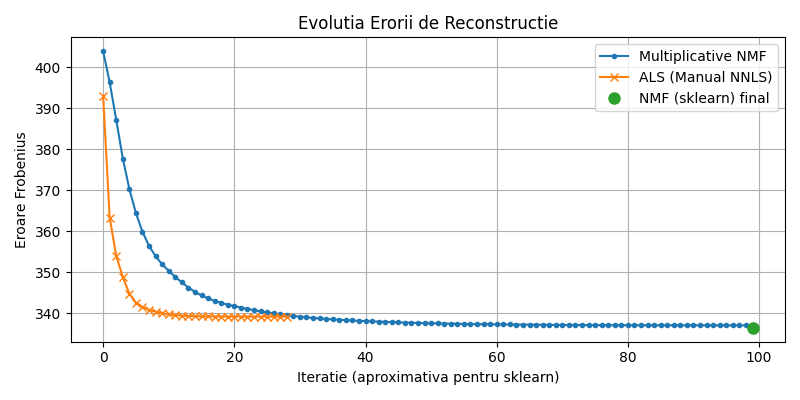
\includegraphics[width=1.0\textwidth]{figure1.png} 
		\caption{Evoluția erorii de reconstrucție pentru diferitele metode de factorizare ($r=10$).}
		\label{fig:error_plot}
	\end{figure}
	
	\subsection{Erori de reconstrucție (Sumar)} 
	Pentru un număr de factori latenti $r=10$, erorile de reconstrucție (norma Frobenius $\|V - WH\|_F$) obținute au fost:
	\begin{itemize}
		\item \textbf{NMF Multiplicativ (Manual):} 337.03
		\item \textbf{NMF (\texttt{sklearn}, solver 'cd'):} 336.42
		\item \textbf{ALS (NNLS Manual):} 339.17
	\end{itemize}
	Rezultatele sunt comparabile, cu implementarea \texttt{sklearn} oferind cea mai mică eroare, urmată îndeaproape de NMF multiplicativ și ALS-NNLS manual.
	
	\subsection{Recomandări generate (Exemplu)}
	\label{subsec:recomandari-exemplu}
	
	Pentru a ilustra tipurile de recomandări generate de fiecare metodă, am selectat piesa de referință \textbf{"Murder One" de Metallica}. Această piesă este un tribut adus lui Lemmy Kilmister de la Motörhead și se încadrează în genul Thrash Metal/Heavy Metal. Mai jos sunt prezentate top 5 recomandări pentru fiecare abordare implementată:
	
	\begin{itemize}
		\item \textbf{Referință: Murder One - Metallica}
		\begin{itemize}
			\item \textit{Recomandări (Tag Similarity - Similaritate Cosinus pe taguri):}
			\begin{itemize}
				\item Necrophiliac - Slayer
				\item Blacklist - Exodus
				\item Electric Crown - Testament
				\item Murder Fantasies - Kreator
				\item Practice What You Preach - Testament
			\end{itemize}
			\vspace{0.5em} 
			\item \textit{Recomandări (NMF Multiplicativ Manual):}
			\begin{itemize}
				\item Crionics - Slayer
				\item Praise of Death - Slayer
				\item Blackmail The Universe - Megadeth
				\item Washington Is Next! - Megadeth
				\item Back In the Day - Megadeth
			\end{itemize}
			\vspace{0.5em}
			\item \textit{Recomandări (NMF \texttt{sklearn}, solver 'cd'):}
			\begin{itemize}
				\item Blacklist - Exodus
				\item At Dawn They Sleep - Slayer
				\item Bite The Hand - Megadeth
				\item Uplift - Pantera
				\item Praise of Death - Slayer
			\end{itemize}
			\vspace{0.5em}
			\item \textit{Recomandări (ALS cu NNLS Manual):}
			\begin{itemize}
				\item Practice What You Preach - Testament
				\item Bite The Hand - Megadeth
				\item Hy Pro Glo - Anthrax
				\item Deviance - Slayer
				\item Tormentor - Slayer
			\end{itemize}
		\end{itemize}
	\end{itemize}
	
	\paragraph{Observații asupra exemplului:}
	Se poate observa că toate metodele tind să recomande piese din subgenuri similare ale metalului (Thrash, Speed, Heavy Metal), ceea ce este de așteptat.
	\begin{itemize}
		\item \textbf{Similaritatea pe taguri} identifică corect piese cu tematici sau stiluri apropiate, menționate explicit în taguri.
		\item \textbf{Metodele de factorizare (NMF și ALS)} generează recomandări care, deși tot din sfera metal, pot proveni de la artiști diferiți, indicând descoperirea unor profiluri latente comune. Prezența consistentă a pieselor de la Slayer, Megadeth, Testament și Anthrax în recomandările bazate pe factorizare sugerează că aceste trupe partajează caracteristici latente similare cu Metallica în contextul datelor analizate.
		\item Diferențele subtile între recomandările NMF și ALS pot fi atribuite modului diferit în care algoritmii converg și ponderează factorii latenti.
	\end{itemize}
	Acest exemplu ilustrează capacitatea metodelor de factorizare de a merge dincolo de potrivirile directe de taguri și de a sugera melodii relevante pe baza unor similarități structurale mai profunde.
	
	\subsection{Timp de execuție și Complexitate Computațională} 
	\begin{itemize}
		\item \textbf{NMF (\texttt{sklearn}):} Cel mai rapid, datorită implementării optimizate și a eficienței algoritmului Coordinate Descent.
		\item \textbf{NMF Multiplicativ (Manual):} Relativ rapid. Fiecare iterație implică operații matriciale, dar nu rezolvarea unor subprobleme de optimizare distincte și complexe.
		\item \textbf{ALS (NNLS Manual):} Cel mai lent. Fiecare iterație a buclei principale ALS necesită rezolvarea a $m+n$ subprobleme NNLS. Deoarece fiecare subproblemă NNLS este rezolvată printr-un algoritm iterativ (proiectarea gradientului), costul computațional total este semnificativ mai mare. Timpul de execuție este direct influențat de \texttt{max\_iter\_als}, \texttt{max\_iter\_nnls} și de eficiența implementării NNLS.
	\end{itemize}
	
	\subsection{Concluzii specifice metodelor}
	\begin{itemize}
		\item Toate cele trei metode de factorizare cu constrângeri de non-negativitate au demonstrat capacitatea de a descompune matricea melodie-tag și de a genera factori latenti utilizabili pentru recomandări, obținând erori de reconstrucție comparabile.
		\item Implementarea din \texttt{sklearn} s-a dovedit a fi cea mai eficientă atât din punct de vedere al erorii finale, cât și al vitezei de execuție.
		\item Implementarea ALS cu NNLS manual, deși mai intensivă computațional, a atins o performanță competitivă după ajustarea parametrilor subproblemelor NNLS. Acest lucru subliniază importanța alegerii corecte a parametrilor (în special rata de învățare și numărul de iterații) pentru algoritmii de optimizare iterativi imbricați.
		\item Metodele de factorizare (NMF și ALS) descoperă similarități latente între melodii, nu doar pe baza tagurilor explicite, ceea ce poate duce la recomandări mai surprinzătoare, diverse și potențial mai relevante pentru utilizator.
	\end{itemize}
	
	\section{Comparare cu alte funcții Python}
	Pentru problema de factorizare non-negativă, funcțiile generice de optimizare cu constrângeri din \texttt{scipy.optimize.minimize} (ex: cu solver-ul 'SLSQP' sau 'L-BFGS-B' cu bounds) ar putea fi teoretic aplicate. Totuși, acestea ar necesita "aplatizarea" matricelor $W$ și $H$ într-un singur vector de variabile, ceea ce ar duce la un număr foarte mare de variabile ($m \times r + r \times n$). Pentru astfel de probleme la scară mare cu structură specifică (factorizare de matrice), algoritmii dedicați precum NMF multiplicativ, Coordinate Descent (din \texttt{sklearn}), sau ALS sunt semnificativ mai eficienți. Am ales să implementăm ALS cu NNLS manual ca o altă metodă specifică problemei, dar care ilustrează optimizarea iterativă a subproblemelor cu constrângeri.
	
	\section{Bibliografie}
	\begin{itemize}
		\item Lee, D. D., \& Seung, H. S. (2001). Algorithms for non-negative matrix factorization. \textit{Advances in neural information processing systems, 13}.
		\item Chih-Jen Lin. (2007). Projected Gradient Methods for Non-negative Matrix Factorization. \textit{Neural Computation, 19(10)}, 2756-2779.
		\item Zdunek, R., \& Cichocki, A. (2007). Non-negative matrix factorization with quadratic programming. \textit{Computers \& Mathematics with Applications, 54(1)}, 70-83.
		\item Berry, M. W., Browne, M., Langville, A. N., Pauca, V. P., \& Plemmons, R. J. (2007). Algorithms and applications for approximate nonnegative matrix factorization. \textit{Computational statistics \& data analysis, 52(1)}, 155-173. (Referință generală bună pentru NMF și aplicații)
		\item \url{https://scikit-learn.org/stable/modules/generated/sklearn.decomposition.NMF.html}
		\item \url{https://en.wikipedia.org/wiki/Non-negative_matrix_factorization}
		\item \url{https://en.wikipedia.org/wiki/Alternating_least_squares}
		\item Hu, Y., Koren, Y., \& Volinsky, C. (2008). Collaborative filtering for implicit feedback datasets. \textit{Eighth IEEE International Conference on Data Mining (ICDM'08)}, 263-272. (Articol clasic despre ALS pentru feedback implicit, relevant pentru contextul general al ALS în recomandări)
	\end{itemize}
	
\end{document}
